\begin{frame}
\frametitle{Прерывания}
\begin{itemize}
    \item<1->Прерывание - это событие, которое заставляет \\
    процессор \emph{прервать} текущую задачу и вызвать \\
    специальный обработчик
    \begin{itemize}
        \item<2-> внешнее устройство требует внимания;
        \item<3-> произошла ошибка при выполнении инструкции;
        \item<4-> специальная инструкция.
    \end{itemize}
\end{itemize}
\end{frame}

\begin{frame}
\frametitle{Асинхронные прерывания}
\begin{itemize}
    \item<1->Прерывания могут происходить асинхронно
    \begin{itemize}
        \item<1->т. е. код не готов к тому, что его прервут
        \item<2->т. е. обработчик прерывания ответственен за
        сохранение состояния прерванной задачи.
    \end{itemize}
\end{itemize}
\end{frame}

\begin{frame}
\frametitle{Обработчики прерываний}
\begin{itemize}
    \item<1-> Откуда берутся обработчики прерываний?
    \begin{itemize}
        \item<2-> часть ядра ОС;
        \item<2-> ОС сообщает процессору, какой обработчик вызывать
        в какой ситуации.
    \end{itemize}
\end{itemize}
\end{frame}

\begin{frame}
\frametitle{Вызов обработчика прерывания}
    \hspace*{\fill}
    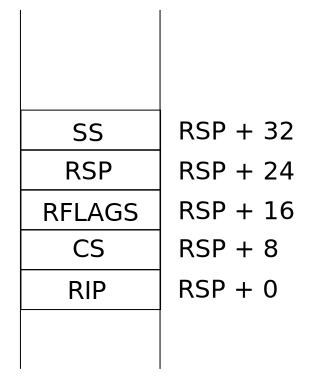
\includegraphics[height=.5\textheight]{intstack}
    \hspace*{\fill}\hspace*{\fill}
\end{frame}

\begin{frame}
\frametitle{Error Code}
\begin{itemize}
    \item<1-> Некоторые прерывания соответствуют ошибочным ситуациям
    \begin{itemize}
        \item<1-> для некоторых из них на стек сохраняется Error Code.
    \end{itemize}
    \item<2-> Error Code \emph{иногда} содержит полезную для обработки
    ошибки информацию
    \begin{itemize}
        \item<3-> а иногда он просто содержит 0.
    \end{itemize}
\end{itemize}
\end{frame}

\begin{frame}
\frametitle{Завершение обработчика прерывания}
\begin{itemize}
    \item<1-> Обработчик прерывания \emph{обычно} завершается
    инструкцией \emph{iretq}
    \begin{itemize}
        \item для прерываний, сохраняющих Error Code, его \emph{необходимо}
        удалить со стека.
    \end{itemize}
\end{itemize}
\end{frame}

\begin{frame}
\frametitle{Тело обработчика прерывания}
\begin{itemize}
    \item<1->В общем случае зависит от прерывания
    \begin{itemize}
        \item например, прерывания от сетевой карты и от таймера требуют
        разной обработки;
    \end{itemize}
    \item<2->Общая часть - сохранение состояния прерванной задачи:
    \begin{itemize}
        \item \emph{RIP} и \emph{RFLAGS} не достаточно;
        \item<3->как минимум, нужно сохранить регистры общего назначения.
    \end{itemize}
\end{itemize}
\end{frame}

\begin{frame}
\frametitle{Таблица дескрипторов прерываний}
\begin{itemize}
    \item<1-> IDT указывает, каким прерываниям какие обработчики соответствуют
    \begin{itemize}
        \item<2-> специальный регистр \emph{IDTR} хранит адрес этой таблицы;
        \item<3-> инструкции \emph{LIDT} и \emph{SIDT} позволяют
        записать/прочитать регистр \emph{IDT}.
    \end{itemize}
\end{itemize}
\end{frame}

\begin{frame}
\frametitle{Дескриптор IDT}
    \hspace*{\fill}
    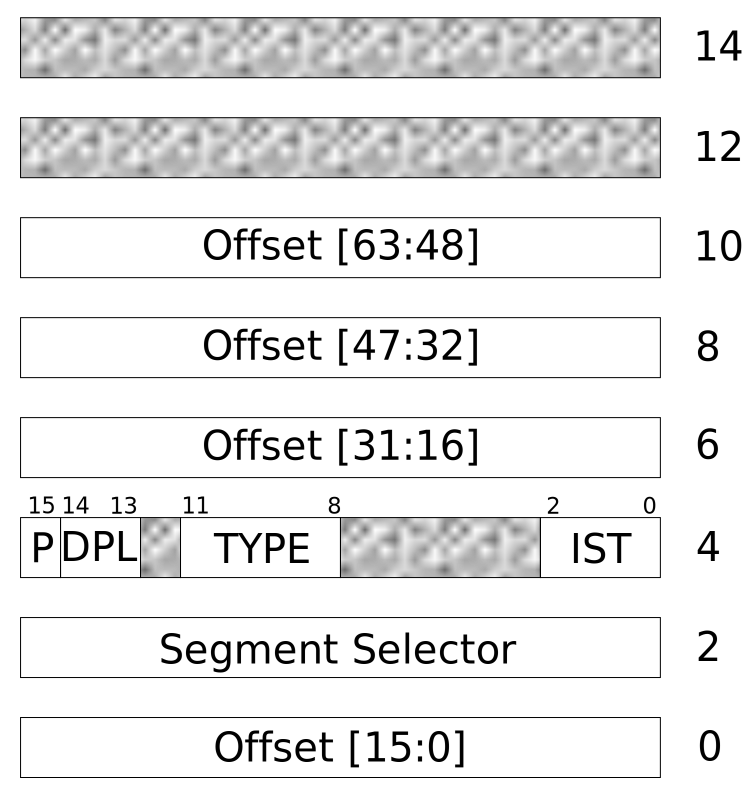
\includegraphics[height=.6\textheight]{desc}
    \hspace*{\fill}\hspace*{\fill}
\end{frame}

\begin{frame}
\frametitle{Таблица дескрипторов прерываний}
\begin{itemize}
    \item<1->IDT может содержать максимум 256 записей
    \begin{itemize}
        \item т. е. каждое ядро может обрабатывать 256 различных прерываний;
        \item<2-> первые 32 из 256 зарезервированы под специальные нужды;
        \item<3-> чему соответствуют оставшиеся 224?
    \end{itemize}
\end{itemize}
\end{frame}

\begin{frame}
\frametitle{Прерывания от внешних устройств}
\begin{itemize}
    \item<1->Какое устройство какую запись в IDT использует?
    \begin{itemize}
        \item<2->может определяться настройкой устройства;
        \item<3->может определяться настройкой контроллера прерываний.
    \end{itemize}
\end{itemize}
\end{frame}

\begin{frame}
\frametitle{Контроллер прерываний}
\begin{itemize}
    \item<1->Контроллер прерываний - посредник между устройствами и процессором
    \begin{itemize}
        \item<2->устройства сигналят контроллеру, контроллер сигналит процессору
        \item<3->задача контроллера - арбитраж (порядок обработки прерываний).
    \end{itemize}
    \item<4->Примеры контроллеров:
    \begin{itemize}
        \item PIC (Programmable Interrupt Controller) (Intel 8259);
        \item APIC (Advanced PIC)(Local APIC + IO APIC).
    \end{itemize}
\end{itemize}
\end{frame}

\begin{frame}
\frametitle{Запрет прерываний}
\begin{itemize}
    \item<1->Зачем запрещать прерывания?
    \begin{itemize}
        \item задача работает с данными, к которым обращается обработчик.
    \end{itemize}
    \item<2->Какие прерывания можно запрещать?
    \begin{itemize}
        \item нельзя запрещать исключения (прерывания из-за ошибок).
    \end{itemize}
\end{itemize}
\end{frame}

\begin{frame}
\frametitle{Запрет прерываний}
\begin{itemize}
    \item<1->Мы можем попросить устройство не генерировать прерывания
    \begin{itemize}
        \item если мы знаем, какие прерывания могут привести к проблемам;
        \item если устройство позволяет.
    \end{itemize}
    \item<2->Отключить прерывание на контроллере прерываний.
\end{itemize}
\end{frame}

\begin{frame}
\frametitle{Запрет прерываний}
\begin{itemize}
    \item<1->Отключить прерывание на процессоре
    \begin{itemize}
        \item<2-> x86 регистр \emph{RFLAGS} содержит флаг \emph{IF};
        \item<3-> инструкция \emph{cli} очищает флаг - запрещает прерывания;
        \item<3-> инструкция \emph{sti} устанавливает флаг.
    \end{itemize}
\end{itemize}
\end{frame}
